\documentclass[8pt,a4paper,compress]{beamer}

\usepackage{/home/siyer/lib/slides}

\title{Binary Search Trees}
\date{}

\begin{document}
\begin{frame}
\vfill
\titlepage
\end{frame}

\begin{frame}
\frametitle{Outline}
\tableofcontents
\end{frame}

\section{What is a Binary Search Tree (BST)?}
\begin{frame}[fragile]
\begin{itemize}
\item a binary tree is either empty or two disjoint binary trees (left and right)

\item a binary tree is in symmetric order if each node has a key and every node's key larger than all keys in its left subtree and smaller than all keys in its right subtree

\item a binary search tree (BST) is a binary tree in symmetric order

\begin{center}
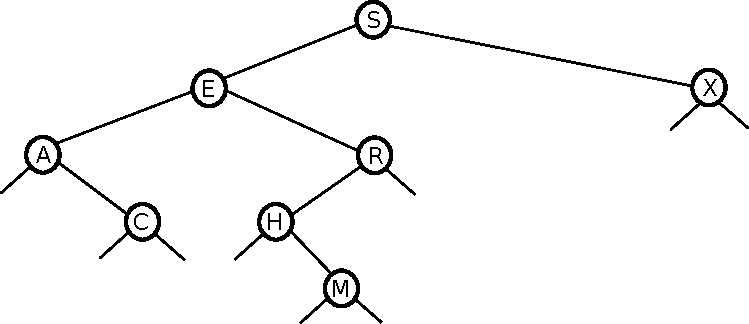
\includegraphics[scale=0.6]{{./figures/bst}.pdf}
\end{center}
\end{itemize}
\end{frame}

\begin{frame}[fragile]
\begin{itemize}
\item a BST representation in Java is a reference to a root node, which is composed of four fields: a key, a value, a reference to the left subtree, a reference to the right subtree, and the number of nodes in the subtree

\begin{lstlisting}[language=Java]
private class Node {
    private Key key; 
    private Value val; 
    private Node left, right; 
    private int N;

    public Node(Key key, Value val, int N) {
        this.key = key;
        this.val = val;
        this.N = N;
    }
}
\end{lstlisting}
\end{itemize}
\end{frame}

\section{Implementation of the Ordered Symbol Table API Using a BST}
\begin{frame}[fragile]
\begin{itemize}
\item basic operations
\begin{lstlisting}[language=Java]
public class BinarySearchTreeST<Key extends Comparable<Key>, Value> 
    implements OrderedST<Key, Value>{
    private Node root;

    private class Node { ... }
    
    public boolean isEmpty() { return size() == 0; }

    public int size() { return size(root); }

    private int size(Node x) {
        if (x == null) { return 0; }
        else return x.N;
    }

    public Value get(Key key) { return get(root, key); }

    private Value get(Node x, Key key) {
        if (x == null) { return null; }
        int cmp = key.compareTo(x.key);
        if      (cmp < 0) { return get(x.left, key); }
        else if (cmp > 0) { return get(x.right, key); }
        else              { return x.val; }
    }

    public boolean contains(Key key) { return get(key) != null; }
    ...
}
\end{lstlisting}
\end{itemize}
\end{frame}

\begin{frame}[fragile]
\begin{itemize}
\item basic operations (contd.)
\begin{lstlisting}[language=Java]
public class BinarySearchTreeST<Key extends Comparable<Key>, Value> 
    ...
    public void put(Key key, Value val) {
        if (val == null) { delete(key); return; }
        root = put(root, key, val);
    }

    private Node put(Node x, Key key, Value val) {
        if (x == null) { return new Node(key, val, 1); }
        int cmp = key.compareTo(x.key);
        if      (cmp < 0) { x.left  = put(x.left,  key, val); }
        else if (cmp > 0) { x.right = put(x.right, key, val); }
        else              { x.val   = val; }
        x.N = 1 + size(x.left) + size(x.right);
        return x;
    }
    ...
}
\end{lstlisting}
\end{itemize}
\end{frame}

\begin{frame}[fragile]
\begin{itemize}
\item tree shape depends on order of insertion

\begin{minipage}{100pt}
\begin{center}
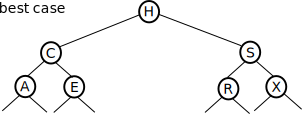
\includegraphics[scale=0.4]{{./figures/bst_possibility1}.pdf}
\end{center}
\end{minipage}%
\begin{minipage}{140pt}
\begin{center}
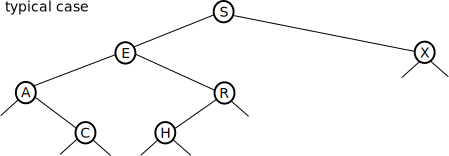
\includegraphics[scale=0.4]{{./figures/bst_possibility2}.pdf}
\end{center}
\end{minipage}%
\begin{minipage}{50pt}
\begin{center}
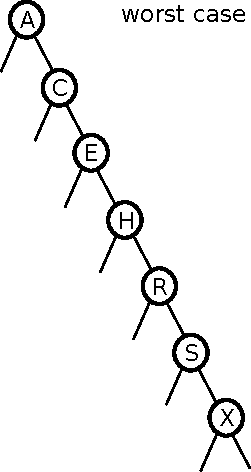
\includegraphics[scale=0.4]{{./figures/bst_possibility3}.pdf}
\end{center}
\end{minipage}

\item number of compares for search/insert is equal to 1 + depth of node

\item if $N$ distinct keys are inserted into a BST in random order,
the expected number of compares for a search/insert is $\sim 2\ln N$
\end{itemize}
\end{frame}

\begin{frame}[fragile]
\begin{itemize}
\item typical BST, built from 256 random keys

\begin{center}
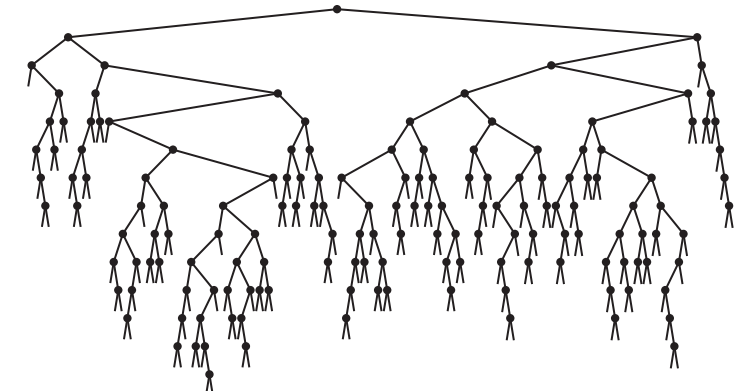
\includegraphics[scale=0.4]{{./figures/typical_bst}.png}
\end{center}
\end{itemize}
\end{frame}

\begin{frame}[fragile]
\begin{itemize}
\item ordered operations
\end{itemize}
\end{frame}

\begin{frame}[fragile]
\begin{itemize}
\item deletion
\end{itemize}
\end{frame}

\section{Performance Characteristics}
\begin{frame}[fragile]
\begin{itemize}
\item 
\end{itemize}
\end{frame}
\end{document}
